% !TEX root = ../main.tex

\section{Analog Front End}
\label{sec:analog-front-end}

\scaffold{
  \textbf{Paragraph 1, the circuit.} Link: \cref{sec:design-history} explained why switches replaced the buffers. Walk through \cref{fig:frontend-final} for one jack, in the order the control signal passes: the 74HC595 \cite{ti2026sn74hc595} (U6) receives the drive pattern over SPI and latches it; its outputs select the switches of U15, which connect a contact to R50 (\qty{1}{\kilo\ohm}, \qty{0.1}{\percent}) and the \qty{2.5}{\volt} rail, and of U19, which connect it to R54 and ground. Each contact reaches its ADC input through R15--R18 (\qty{10}{\kilo\ohm}) with C23--C26 (\qty{10}{\nano\farad}) to ground. The four shift registers form one chain from the microcontroller to the fourth jack; their output enable is pulled high, so all switches stay open until the firmware writes the first pattern. Mention that the drive enum in the firmware makes it impossible to close the pull-up and pull-down switch of one contact at the same time.
}

\begin{figure}[htbp]
  \centering
  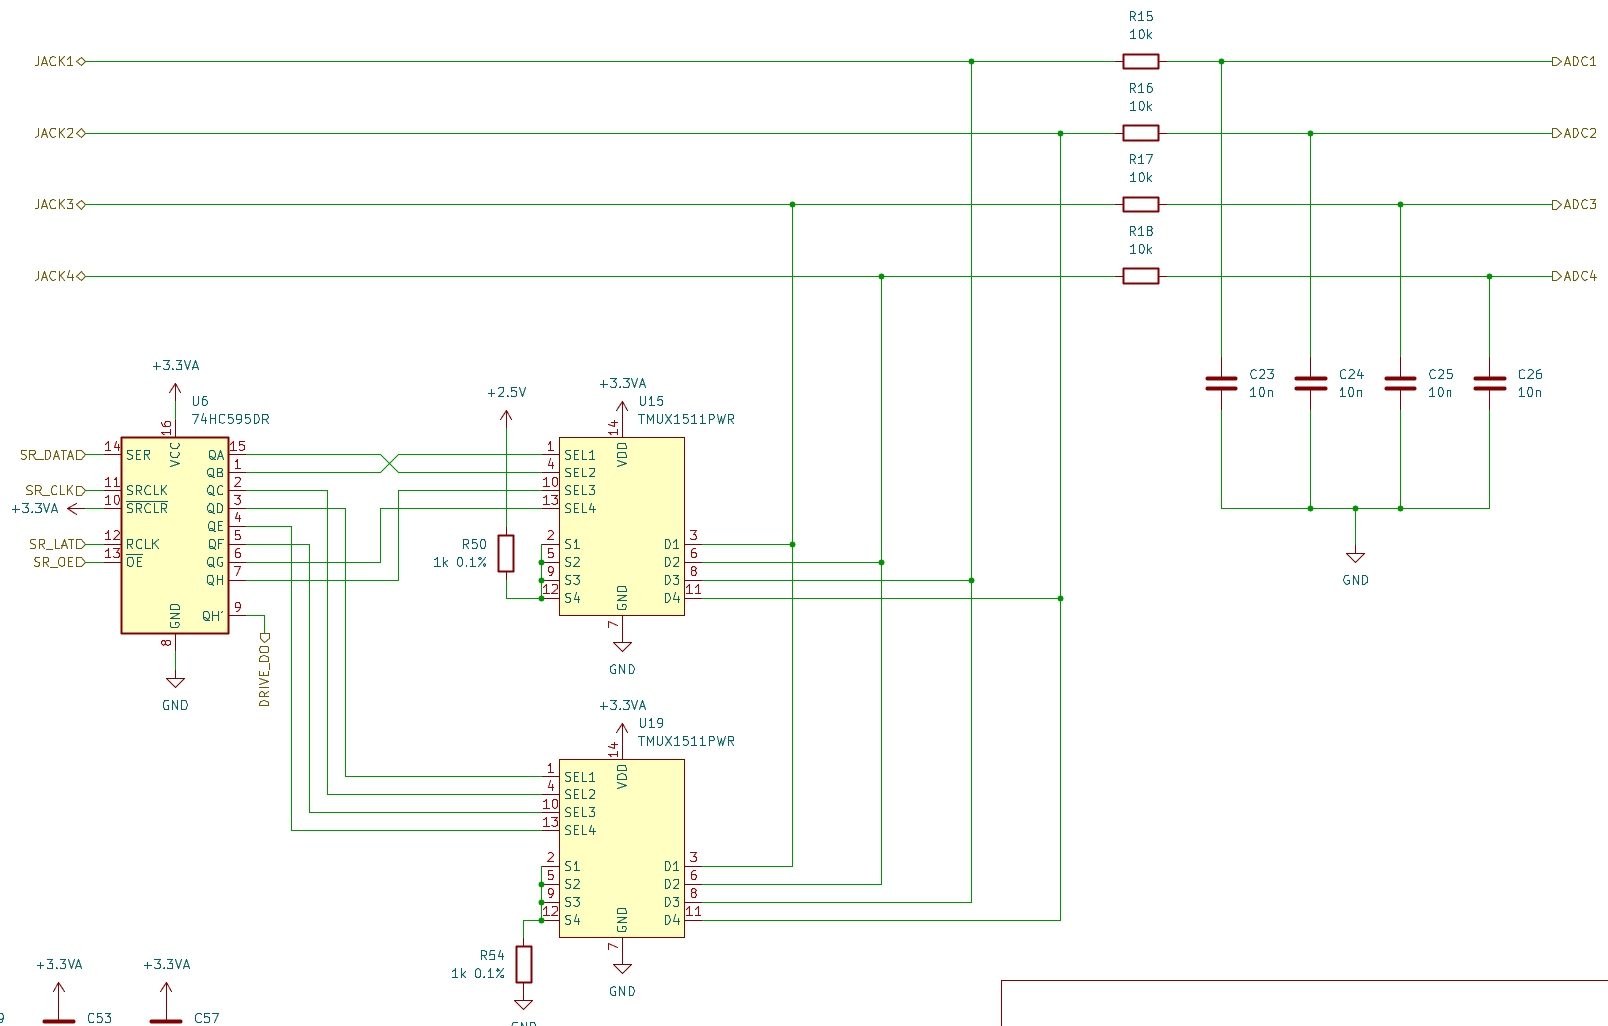
\includegraphics[width=\linewidth]{04-implementation/figures/frontend-final}
  \titledcaption{Analog Front End of One Jack}{\scaffoldinline{Name U6, U15, U19, R50, R54, R15--R18 and C23--C26 and their role; explain that JACK1--JACK4 are the four contacts of one jack (tip, ring, sleeve, tip switch, check the order against \code{src/board.rs}) and ADC1--ADC4 their ADC inputs. Source: KiCad sheet \code{hardware/AnalogQuadChannel.kicad\_sch}.}}
  \label{fig:frontend-final}
\end{figure}

\scaffold{
  \textbf{Paragraph 2, settling.} When the drive pattern changes, a floating contact charges the filter capacitor through the pedal and the filter resistor. Present \cref{eq:settling}: the firmware waits two time constants, between \qty{1}{\milli\second} and \qty{400}{\milli\second}, with $R_\mathrm{net}$ the resistance of the network through which the floating contact charges, known from the previous solve (an unknown network is assumed to be \qty{100}{\kilo\ohm}). Compute $\tau$ for a \qty{10}{\kilo\ohm} pedal (about \qty{0.2}{\milli\second}) and a \qty{500}{\kilo\ohm} pedal (about \qty{5}{\milli\second}). Refer to \cref{sec:results-settling} for the measured time constant.
}

\begin{equation}
  t_\mathrm{settle} = 2\,\tau,
  \qquad
  \tau = \bigl(R_\mathrm{net} + R_\mathrm{f}\bigr)\,C_\mathrm{f},
  \qquad
  \qty{1}{\milli\second} \leq t_\mathrm{settle} \leq \qty{400}{\milli\second}
  \label{eq:settling}
\end{equation}

\scaffold{
  \textbf{Paragraph 3, choice of the pull resistance.} The pull resistance trades position resolution against current resolution: across a pedal of resistance $R$ lies $U\,R/(R + 2R_\mathrm{p})$, across each pull resistor $U\,R_\mathrm{p}/(R + 2R_\mathrm{p})$. Present \cref{tab:pull-resistance} and draw the conclusion: the position uses the span and is fine with any value; only the total resistance of high-value pedals depends on the drop. With \qty{1}{\kilo\ohm} and \qty{0.4}{\milli\volt} noise every pedal up to about \qty{500}{\kilo\ohm} still resolves; \qty{4.7}{\kilo\ohm} would be the value to fit if accurate totals of 250 to \qty{500}{\kilo\ohm} pedals mattered (\cref{ch:conclusion}).
}

\begin{table}[htbp]
  \centering
  \titledcaption{Voltage Span and Pull Drop}{\scaffoldinline{Explain that each cell gives the voltage across the pedal and the drop across one pull resistor for a \qty{2.5}{\volt} rail; the fitted value is \qty{1}{\kilo\ohm}. Source: \code{docs/fast-tracking.md}.}}
  \label{tab:pull-resistance}
  \begin{tabular}{@{}l *{3}{c}@{}}
    \toprule
    \textbf{Pull resistance} & \textbf{\qty{10}{\kilo\ohm} pedal} & \textbf{\qty{100}{\kilo\ohm} pedal} & \textbf{\qty{500}{\kilo\ohm} pedal} \\
    \midrule
    \qty{1}{\kilo\ohm} (fitted) & \qty{2.08}{\volt} / \qty{208}{\milli\volt} & \qty{2.45}{\volt} / \qty{24}{\milli\volt} & \qty{2.49}{\volt} / \qty{5}{\milli\volt} \\
    \qty{2.2}{\kilo\ohm} & \qty{1.74}{\volt} / \qty{382}{\milli\volt} & \qty{2.40}{\volt} / \qty{53}{\milli\volt} & \qty{2.48}{\volt} / \qty{11}{\milli\volt} \\
    \qty{4.7}{\kilo\ohm} & \qty{1.29}{\volt} / \qty{606}{\milli\volt} & \qty{2.29}{\volt} / \qty{107}{\milli\volt} & \qty{2.45}{\volt} / \qty{23}{\milli\volt} \\
    \qty{10}{\kilo\ohm} & \qty{0.83}{\volt} / \qty{833}{\milli\volt} & \qty{2.08}{\volt} / \qty{208}{\milli\volt} & \qty{2.45}{\volt} / \qty{49}{\milli\volt} \\
    \bottomrule
  \end{tabular}
\end{table}

\openquestion{Choice of 1 kOhm}{
  Was \qty{1}{\kilo\ohm} chosen with the analysis of \cref{tab:pull-resistance} in mind, or was the analysis done afterwards on the finished board? The answer decides whether paragraph~3 describes a design decision or a later evaluation.
}
